\chapter{Setting up the $HH\rightarrow \bbbb$ Analysis}
\label{chap:bbbb-intro}

The following chapters present two complementary searches for pair production of 
Higgs bosons in the $\bbbb$ final state. Such searches are separated based on the 
signal models being considered: resonant production, in which a new spin-0 or 
spin-2 particle is produced and decays to two Standard Model Higgs bosons, and 
non-resonant production, which is sensitive to the value of the Higgs self-coupling
$\lambda_{HHH}$. Further information on the theory behind both channels can be 
found in Chapter \ref{chap:hh-bsm}.

ATLAS has performed a variety of searches for both resonant and non-resonant $HH$ in complementary 
decay channels, notably for early Run 2 in the $\bbbar\Wplus\Wminus$~\cite{HIGG-2016-27},
$\bbbar\tautau$~\cite{HIGG-2016-16},
$\Wplus\Wminus\Wplus\Wminus$~\cite{HIGG-2016-24},
$\bbbar\gamma\gamma$~\cite{HIGG-2016-15}, and
$\Wplus\Wminus\gamma\gamma$~\cite{HIGG-2016-20} final states, which were combined
along with $\bbbar\bbbar$ in~\cite{HDBS-2018-58}. ATLAS has also released 
a variety of full Run 2 results, including boosted $\bbbar\tautau$~\cite{HDBS-2019-22}, 
VBF $\bbbb$~\cite{HDBS-2018-18}, $\bbbar\ell\nu\ell\nu$~\cite{HDBS-2018-33}, and 
$\bbbar\gamma\gamma$~\cite{ATLAS-CONF-2021-016}.

CMS has also performed searches for production of Higgs boson pairs in
the $\bbbar\bbbar$ final state (among others) for early Run 2~\cite{CMS-B2G-17-019} and 
full Run 2~\cite{CMS-PAS-HIG-20-005}. A combination of CMS searches in the 
$\bbbar\bbbar$, $\bbbar\tautau$, $\bbbar\gamma\gamma$, and $\bbbar\VVbos$ channels 
was performed for early Run 2 in~\cite{CMS-HIG-17-030}.

While the resonant and non-resonant searches presented here face many similar challenges and 
proceed (in broad strokes) in a very 
similar manner, separate optimizations are performed to maximize the respective sensitivities 
for these two very different sets of signal hypotheses. More particularly, resonant signal 
hypotheses are (1) very peaked in values of the mass of the $HH$ candidate system near the 
value of the resonance mass considered and (2) considered across a very broad range of 
signal mass hypotheses. The resonant searches are therefore split into resolved and boosted 
topologies based on Lorentz boost of the decay products, with the resolved channel as one of the 
primary focuses of this thesis. Further, several analysis design decisions are made to 
allow for sensitivity to a broad range of masses -- in particular, though sensitivity is 
limited at lower values of \mhh relative to other channels (see, e.g. Chapter \ref{chap:compare}) 
due to the challenging background, retaining and properly reconstructing these low mass events 
allows the \bbbb channel to retain sensitivity as low as the kinematic threshold at \SI{250}{\GeV}.

In contrast, non-resonant signal hypotheses are quite broad in \mhh, and have a much more limited 
mass range, with Standard Model production peaking near \SI{400}{GeV}, and the majority of the analysis 
sensitivity able to be captured with a resolved topology. Even for Beyond the Standard 
Model signal hypotheses, which may have more events at low \mhh, the non-resonant nature of the
production allows the \bbbb channel to retain sensitivity while discarding much of the challenging 
low mass background. Such freedom allows for decisions which focus on improved background modeling 
for the middle to upper $HH$ mass regime, resulting in improved modeling and smaller uncertainties 
than would be obtained with a more generic approach.

Both searches are presented in the following, with emphasis on particular motivations for, and consequences
of, the various design decisions involved for each respective set of signal hypotheses. A comparison of 
representative signals for both the resonant and non-resonant analyses is shown in Figure \ref{fig:sig-examples}.

\begin{figure}[ht]
\centering
\subfloat{
		  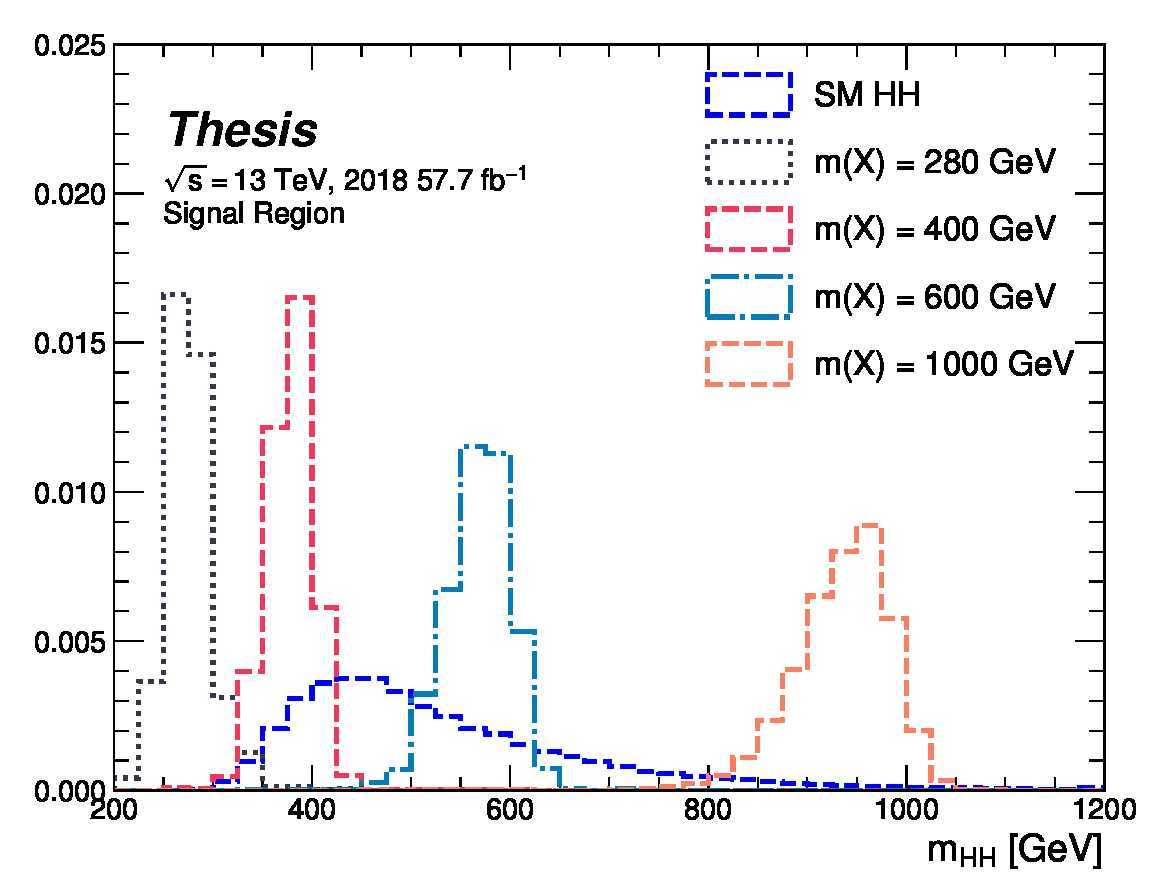
\includegraphics[width=0.8\textwidth]{figures/signal-example-plot.pdf}
		 }
\caption{\label{fig:sig-examples} Example distributions in invariant mass of the reconstructed di-Higgs system 
for a variety of spin-0 resonances ($m(X)$) compared to the Standard Model non-resonant signal (SM HH). 
Both are presented in their respective signal regions, after all corresponding analysis selections. The resonant 
signals are sharply peaked at values near their respective resonance masses, whereas the non-resonant signal is much 
more broad. The different character of these different signals informs the analysis design.}
\end{figure}


The analyses improve upon previous work~\cite{EXOT-2016-31} in several notable ways. The resonant search leverages 
a Boosted Decision Tree (BDT) based algorithm for the reconstruction of the $HH$ system from the jets considered for 
the analysis, offering an improved efficiency of that reconstruction over a broad mass spectrum. The non-resonant 
adopts a different approach, with 
a simplified algorithm based on the minimum angular distance ($\Delta R$) between jets in a reconstructed 
Higgs candidate. Such an approach very efficiently discards low mass background events, resulting in an 
easier to estimate background with reduced systematic uncertainties.

A particular contribution of this thesis is the background estimation, which uses a novel, neural network
based approach to perform a data-driven estimation of the background, which is dominated by QCD processes, for which 
a sufficient simulation is not available. This new approach offers improved modeling over previous methods, as 
well as the ability to model correlations between observables. While all aspects of the analysis of course contribute 
to the final result, the author of this 
thesis wishes to emphasize that the background estimate, with the corresponding uncertainties and all 
other associated decisions, really is the core of the $HH\rightarrow \bbbb$ analysis -- the development
of this procedure, and all associated decisions, is similarly the core of this thesis work.


This analysis also benefits from improvements to ATLAS jet reconstruction and
calibration, and flavor tagging~\cite{FTAG-2018-01}. In particular, this
analysis benefits from the introduction of particle flow
jets~\cite{PERF-2015-09}. These make use of tracking information to supplement
calorimeter energy deposits, improving the angular and transverse momentum
resolution of jets by better measuring these quantities for charged particles in
those jets.

The analysis also benefits from the new DL1r ATLAS flavor tagging algorithm.
Whereas the flavor tagging algorithm used in the previous analysis (MV2) used a
boosted decision tree (BDT) to combine the output of various low level
algorithms, DL1r (and the baseline DL1 algorithm) uses a deep neural network to
do this combination. In addition to the low level algorithms used as inputs to
MV2, DL1 includes a variety of additional variables used for $\Pqc$-tagging. DL1r
further incorporates RNNIP, a recurrent neural network designed
to identify \bjets using the impact parameters, kinematics, and quality
information of the tracks in the jets, while also taking into account the
correlations between the track features.

The overall analysis sensitivity further benefits from a factor of 
4.6 increase in integrated luminosity.

\section{Data and Monte Carlo Simulation}
Both the resonant and non-resonant searches are performed on the full ATLAS Run 2 dataset, consisting of 
$\sqrt{s} = \SI{13}{\TeV}$ proton-proton collision data taken from 2016 to 2018 inclusive. Data taken in 2015 
is not used due to a lack of trigger jet matching
information and \bjet trigger scale factors\footnote{These trigger scale factors account for differences 
in the performance of the b-tagging algorithms between simulation and data, with the jet matching providing a 
correspondence between the jets in the trigger decision and the jets in the offline analysis}. The integrated 
luminosity collected
and usable in this analysis\footnote{\label{foot:lost-lumi}approximately
  \SI{9}{\ifb} of data was collected but could not be used in this analysis due
  to an inefficiency in the \bjet triggers at the start of 2016~\cite{ATL-COM-DAQ-2019-150}} was:
\begin{itemize}
  \item \SI{24.6}{\ifb} in 2016
  \item \SI{43.65}{\ifb} in 2017
  \item \SI{57.7}{\ifb} in 2018
\end{itemize}

This gives a total integrated luminosity of \SI{126}{\ifb}.
This is lower than the \SI{139}{\ifb} ATLAS collected during \RunTwo
\cite{ATLAS-CONF-2019-021} due to the inefficiency described in
footnote~\ref{foot:lost-lumi} as well as the \SI{3.2}{\ifb} 
of 2015 data which is unused due to the trigger scale factor 
issue mentioned above.

In this analysis, Monte Carlo samples are used purely for modelling signal
processes. The background is strongly dominated by events produced by QCD
multijet processes, which are difficult to correctly model in simulation due to 
the complexity of the interactions involved (including, e.g. non-perturbative effects), as well as the harsh requirement 
of four $b$-tagged jets, which makes it difficult to collect sufficient Monte Carlo statistics. This
necessitates the use of a data-driven background modeling technique, which is
described in Chapter \ref{chap:bbbb-background}.

The scalar resonance signal model is simulated at leading order in \alphas using
\MADGRAPH\cite{MG5}. Hadronization and parton showering are done using
\HERWIG[7]~\cite{Herwig7}\cite{HerwigPP} with \textsc{EvtGen}~\cite{EvtGen},
and the nominal PDF is NNPDF 2.3 LO. In practice this is implemented as a two
Higgs doublet model where the new neutral scalar is produced through gluon
fusion and required to decay to a pair of SM Higgs bosons. The heavy scalar is
assigned a width much smaller than detector resolution, and the other 2HDM
particles do not enter the calculation.

Scalar samples are produced at resonance masses between \SIlist{251;900}{\GeV} and the detector
simulation is done using AtlFast-II~\cite{SOFT-2010-01}. In addition the samples at \SI{400}{\GeV}
and \SI{900}{\GeV} are also fully simulated to verify that the use of AtlFast-II
is acceptable. For higher masses, as well as for the boosted analysis, 
samples are produced between \SIlist{1000;5000}{\GeV}, and the detector is fully simulated.
As discussed in Chapter \ref{chap:simulation}, an outstanding issue with AtlFast-II is the 
modeling of jet substructure. While such variables are not used for the resolved analysis,
the boosted analysis begins at $\SI{900}{\GeV}$, motivating the different detector 
simulation in these two regimes.

The spin-2 resonance signal model is also simulated at LO in \alphas using
\MADGRAPH. Hadronization and parton showering are done using
\PYTHIA[8]~\cite{Pythia} with \textsc{EvtGen}, and the nominal PDF is NNPDF 2.3
LO. In practice this is implemented as a Randall-Sundrum graviton with $c=1.0$.

Spin-2 resonance samples are produced at masses between \SIlist{251;5000}{\GeV}, 
and these samples are all produced with full detector simulation.

For the non-resonant search, samples are produced at values of $\kappa_{\lambda} = 1.0$ and $10.0$, and are simulated
using \POWHEGBOX v2 generator~\cite{Powheg1, Powheg2, Powheg3} at next-to-leading order (NLO), with full 
NLO corrections with finite top mass, using the PDF4LHC~\cite{Butterworth:2015oua} parton distribution 
function (PDF) set. Parton showers and hadronization are simulated with \PYTHIA[8].


\section{Triggers}
\label{sec:trigger}
To maximize analysis sensitivity, a combination of multi-\Pqb-jet triggers is used. Due to the 
use of events with two \Pqb-tagged jets in the background estimate, such triggers have a maximum 
requirement of two \Pqb-tagged jets. For the resonant analysis, a combination of triggers of 
various topologies is used, namely
\begin{itemize}
	\item 2b + HT, which requires two $b$-tagged jets and a minimum value of of $H_{T}$, defined to be the scalar sum of $p_{T}$ across all jets in the event.
	\item 2b + 2j, which requires two $b$-tagged jets and two other jets matching some kinematic requirements
	\item 2b + 1j, which requires two $b$-tagged jets and one other jet matching some kinematic requirements
	\item 1b, which requires one $b$-tagged jet
\end{itemize}
Due to minimal contributions from some of these triggers for the Standard Model non-resonant signal, a simplified strategy relying entirely on $2b+1j$ and $2b+2j$ triggers is used for the non-resonant search.

While the use of multiple triggers is beneficial for analysis sensitivity, it comes with some
complications. Namely, a set of scale factors must be assigned to simulated events to 
account for differences in trigger efficiency between real and simulated events. Because these scale 
factors may differ between triggers, the use of multiple triggers becomes complicated: an event may pass 
more than one trigger,while trigger scale factors are only provided for individual triggers.

To simplify this calculation, a set of hierarchical offline selections is applied, closely 
mimicking the trigger selection. Based on these selections, events are sorted into categories
(\emph{trigger buckets}), after which the decision of a \emph{single trigger} is checked. Note 
that the set of events which enter the analysis via this trigger category selection must pass both the 
offline selection as well as the corresponding online trigger selection. Particularly for the $2b$ 
categories, this means that the explicit requirement of two $b$-tagged jets is left to the trigger decision 
itself, with the categorization designed around the other considered objects (non-tagged jets or $H_{T}$).

The resonant search applies such categorization in the following way, with 
selections considered in order:
\begin{enumerate}
	\item If the leading jet is $b$-tagged with $p_{T} > \SI{325}{\GeV}$, the event is in the $1b$ trigger category.
	\item Otherwise, if the leading jet is not $b$-tagged, but has $p_{T} > \SI{168.75}{\GeV}$, the event is in the $2b+1j$
	trigger category.
	\item If neither of the first two selections pass, if the scalar sum of jet $p_{T}$s, $H_{T} > \SI{900}{\GeV}$,
	the event falls into the $2b+HT$ trigger category.
	\item Events that do not pass any of the above offline selections are in the $2b+2j$ trigger category.
\end{enumerate}
Corresponding triggers are then checked in each category, and the final set of events consists of those events that 
pass the trigger decision in their respective categories. 

For the resonant search, the $2b+1j$ and $2b+2j$ triggers are the dominant categories, containing roughly 26~\% and
49~\% of spin-2 events, evaluated on MC16d samples with resonance masses between \SIlist{300;1200}{\GeV}. Notably, 
the $1b$ trigger efficiency is largest at high $(>\SI{1}{\TeV})$ resonance masses.

For the non-resonant search, it was noted that the $1b$ trigger has minimal contribution, while the $2b+HT$ events are 
largely captured by the $2b+2j$ trigger. Therefore, a simplified scheme is considered, 
with selections:
\begin{enumerate}
	\item If the 1st leading jet has $p_{T} > \SI{170}{\GeV}$ and the 3rd leading jet has $p_{T} > \SI{70}{\GeV}$,
	the event is in the $2b+1j$ trigger category.
	\item Otherwise, the event is in the $2b+2j$ trigger category.
\end{enumerate}
The additional cut (on the 3rd leading jet) added here for the $2b+1j$ category was found to enhance the overall 
signal yield in the two bucket strategy relative to the single cut on leading jet $p_{T}$ used for the same category 
in the resonant strategy.
